\subsection{Descri\c c\~ao das Etapas}

\textbf{An\'alise explorat\'oria dos dados (EDA)}
a partir da \ref{etp:1}, foi realizado o EDA (do inglês \textit{Exploratory Data Analysis}) para processar os dados obtidos até o momento. A análise exploratória de dados foi promovida por John Tukey \cite{Bandara2021} como uma abordagem para explorar os dados, resumir suas principais características e formular hipóteses que possam direcionar a coleta adicional de dados e experimentos. No contexto de análises de dados, várias técnicas de EDA têm sido adotadas.
Nessa análise da EDA, serão abordadas várias análises, como a correlação de Pearson, para iniciar e verificar quais variáveis podem ser excluídas como ruído e não têm correlação com a variável LT01. Nesse caso, as variáveis retiradas são consideradas negativas e têm pouca correlação com o LT01, as únicas variáveis que apresentam correlação negativa são B3 e FT02, mesmo sendo uma correlação negativa, essas variáveis possuem uma correlação inviável ou próxima de $0$, levando à decisão de removê-las.

Uma análise bem feita do EDA mostra tudo que os dados podem ter. Esses dados fornecidos pela companhia SANEPAR são coletados em campo por hora, como por exemplo, a cada hora possui um valor esperado. Nisso, pode haver os famosos NaN, que representam a falta de dado coletado, como em um dia em que as bombas podem ter ido para manutenção. Esses NaNs também podem ser registrados como uma anomalia nos dados.

A Figura \ref{fig:person} mostra a correlação entre as variáveis no conjunto de dados em questão. Essa imagem representa graficamente a relação entre as variáveis e é usada para evidenciar a existência de uma correlação forte no valor de $0,97$ é considerada forte entre elas, quanto mais próximo do valor $1$ a correlação é sempre forte e $0,9$ para mais ou para menos indica uma correlação muito forte, 0 a $0,3$ positivo ou negativo indica uma correlação desprezível.

\begin{figure}[!htb]
	\centering
	\caption{Correlação de Pearson}
	\label{fig:person}
	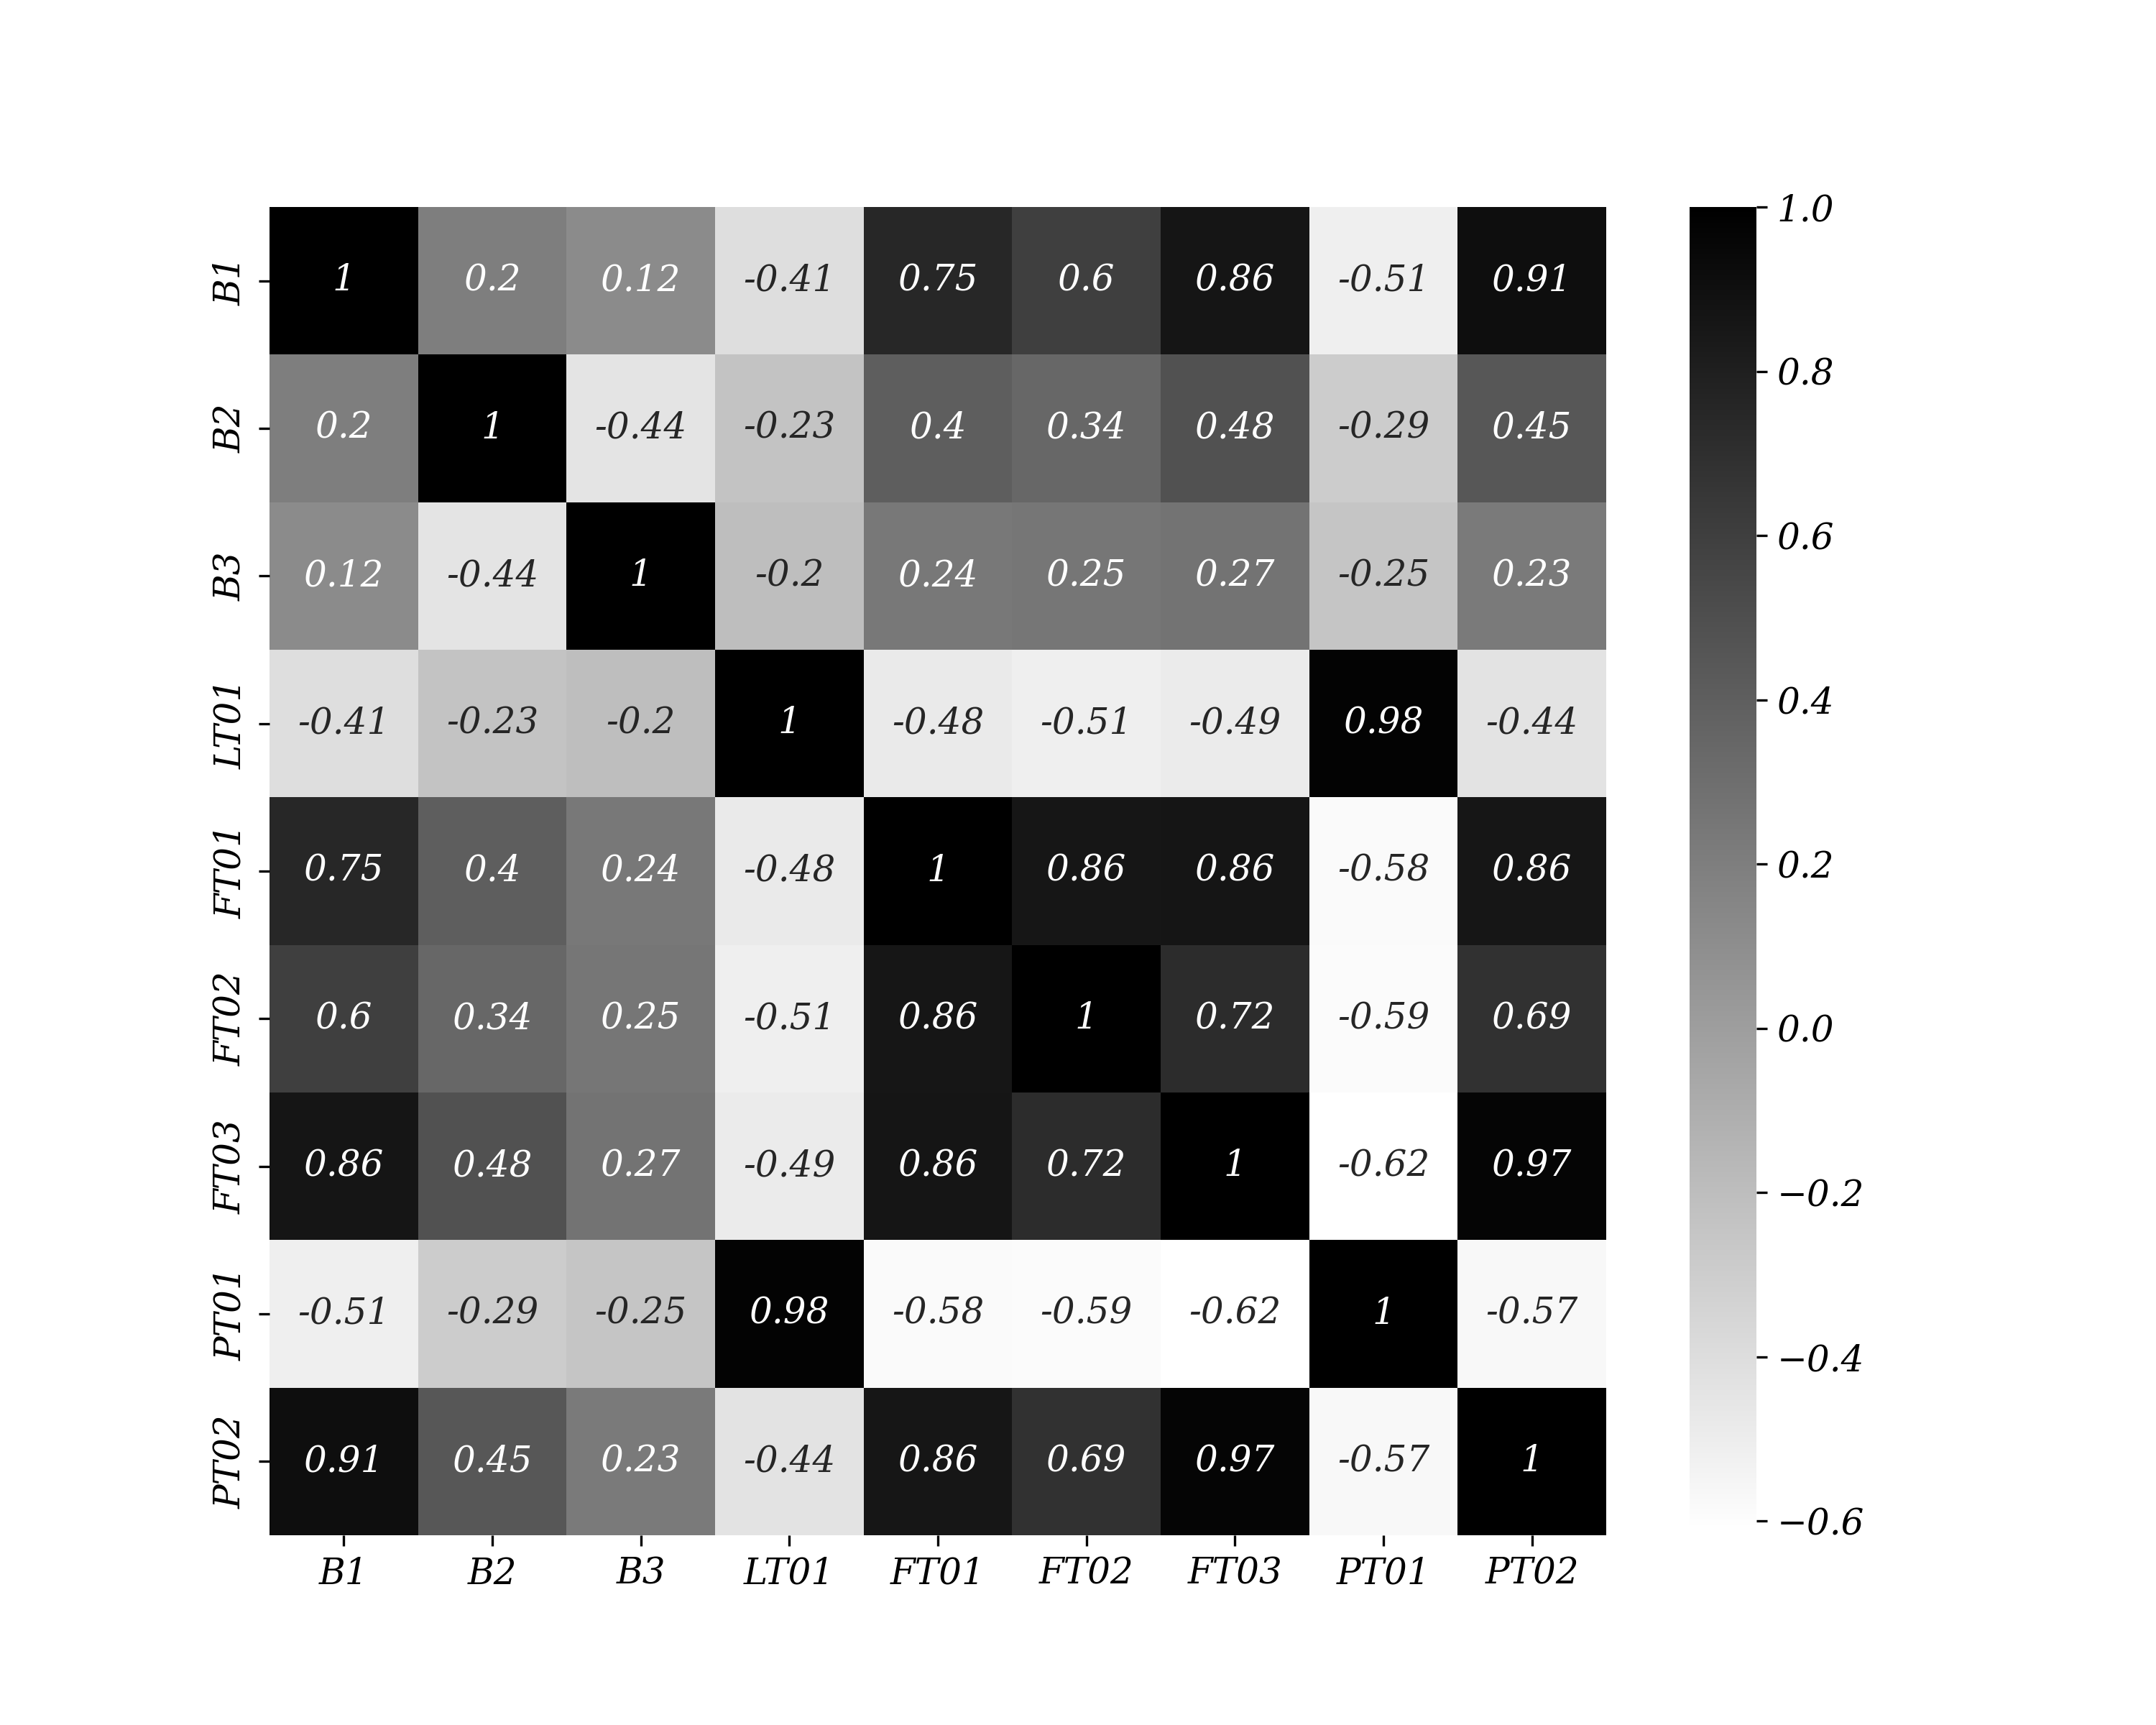
\includegraphics[width=0.7\linewidth]{Apendices/Figuras/modelagem-24h/person}
	
	
\end{figure}

Nesse conjunto de dados que está sendo trabalhado, há uma forte correlação da variável PT01 nos modelos de LR e DTR (do inglês \textit{Decision Tree Regressor}). Esses modelos foram escolhidos para trabalhar com o LT01 como entrada e o PT01 como saída. A Figura \ref{fig:lr-lt01-m3} fornece uma representação dos coeficientes $\beta_0$ e $\beta_1$. Um aumento de $1$ na variável $x$ está associado a um aumento proporcional de $\beta_1$ na variável $y$. O valor de $\beta_0$ representa o valor de $y$ quando $x$ é igual a $0$.

\begin{figure}[!htb]
	\centering
	\caption{Regressão linear LT01 vs PT01 correlação 97\%}
	\label{fig:lr-lt01-m3}
	\includegraphics[width=0.7\linewidth]{"Modelos/Figuras/LR LT01 (m³)"}
	
	
\end{figure}

%Na análise de correlação de Pearson, todo o conjunto de dados da SANEPAR foi utilizado para que cada variável pudesse ser avaliada quanto à sua correlação com a variável LT01. Se houvesse correlação, a variável era usada como variável exógena para melhorar os modelos. Como o modelo de LR consegue relacionar apenas uma ou duas variáveis entre si, no modelo de LR, LT01 foi usada como variável independente e PT01 como variável dependente.






A Tabela \ref{tb:est}, o desvio padrão é representado pela sigla STD, que corresponde à expressão em inglês \textit{standard deviation}. Assim como em qualquer empresa de tratamento de água, é utilizado um mecanismo de acionamento automático denominado ``trava de segurança'' para evitar que o nível do tanque se aproxime de zero e haja falta de água nos locais abastecidos por esse tanque. O nível máximo que o tanque pode alcançar é de $5,26 m^3$ (equivalente a $5264.56$ litros). As bombas são ativadas em sua potência máxima para evitar que sejam acionadas quando o nível do tanque estiver dentro dessa faixa. No entanto, a bomba $1$ ainda estaria operando para completar o nível do tanque caso esteja dentro dessa faixa. Nessa Tabela \ref{tb:est}, foram filtrados os horários de pico nos quais pode ocorrer a maior demanda d'água.

\begin{table}[!htb]
	\centering
	\caption{Descrição estatística dos dados com o filtro aplicado das 18h às 21h}\label{tb:est}
	\begin{tabular}{@{}cccccccccc@{}}
\toprule
\multicolumn{1}{l}{\textbf{18h a 21h}} & \multicolumn{1}{c}{\textbf{B1}} & \multicolumn{1}{c}{\textbf{B2}} & \multicolumn{1}{c}{\textbf{B3}} & \multicolumn{1}{c}{\textbf{LT01}} & \multicolumn{1}{c}{\textbf{FT01}} & \multicolumn{1}{c}{\textbf{FT02}} & \multicolumn{1}{c}{\textbf{FT03}} & \multicolumn{1}{c}{\textbf{PT01}} & \multicolumn{1}{c}{\textbf{PT02}} \\ \midrule
\textbf{Contagem}                      & 2921                            & 2921                            & 2921                            & 2921                              & 2921                              & 2921                              & 2921                              & 2921                              & 2921                              \\
\textbf{Média}                         & 55,98                           & 30,60                           & 5,26                            & 3,18                              & 86,52                             & 132,87                            & 117,62                            & 4,04                              & 22,55                             \\
\textbf{STD}                           & 10,00                           & 15,63                           & 15,57                           & 0,67                              & 124,41                            & 18,48                             & 12,83                             & 0,71                              & 2,92                              \\
\textbf{Min.}                          & 0                               & 0                               & 0                               & 0,29                              & 0                                 & 0                                 & 0,03                              & 0,88                              & 0                                 \\
\textbf{25\%}                          & 57,99                           & 31,63                           & 0                               & 2,77                              & 0                                 & 123,40                            & 112,52                            & 3,61                              & 21,98                             \\
\textbf{50\%}                          & 57,99                           & 35,20                           & 0                               & 3,24                              & 0,12                              & 132,88                            & 118,18                            & 4,10                              & 22,87                             \\
\textbf{75\%}                          & 57,99                           & 38,17                           & 0                               & 3,71                              & 258,48                            & 142,89                            & 124,48                            & 4,59                              & 23,05                             \\
\textbf{Max.}                          & 59,99                           & 59,99                           & 59,99                           & 4,39                              & 370,35                            & 277,94                            & 167,78                            & 5,31                              & 28,08                             \\ \bottomrule
	\end{tabular}
	
	
\end{table}



A realização da EDA consegue mostrar que os dados estão sendo coletados de maneira significativa, ao observar as correlações e possibilita trabalhar com as variáveis que apresentam correlação maior ou não negativa. Nos modelos ARIMA e seus antecessores, ele utiliza o ACF (do inglês \textit{\textit{Auto-Correlation Function}}) e o PACF (do inglês \textit{Partial Auto-correlation Function}) para analisar esses métodos. A análise destes métodos para o modelo ARIMA permite otimizar os parâmetros do modelo.

O ACF é uma medida estatística utilizada para identificar a presença de correlação serial em uma série temporal. Ele calcula a autocorrelação entre os valores da série em diferentes defasagens, ou seja, a correlação entre os valores atuais e os valores passados da série. 

O ACF é útil para analisar a dependência temporal dos dados e identificar padrões de sazonalidade, tendência ou outros efeitos temporais. Por meio do ACF, é possível avaliar se a série exibe autocorrelação significativa em defasagens específicas, o que pode indicar a presença de não estacionariedade ou estrutura temporal que precisa ser considerada na análise ou modelagem da série temporal.


A estatística ADF (do inglês \textit{Augmented Dickey-Fuller}) de $-12,515$ indica a evidência de estacionariedade na série temporal. Quanto mais negativo for o valor da estatística ADF, maior é a evidência de estacionariedade nos dados.

O valor de p, aproximadamente de $0,0000000000000000000000262$, expresso de forma mais concisa como $2,62\times 10^{-23}$ usando a notação científica, está associado ao teste ADF. Este valor-p representa a probabilidade de obter um resultado igual ou mais extremo do que o observado, sob a suposição de que a hipótese nula seja verdadeira. No contexto do teste ADF, a hipótese nula é a presença de raiz unitária na série temporal, indicando não estacionariedade. Portanto, um valor de p baixo, geralmente abaixo de um nível de significância predefinido, como $0,05$, sugere que a série temporal é estacionária, enquanto um valor de p alto sugere não estacionariedade. Dado o valor de p de $2,62\times 10^{-23}$, evidencia-se uma probabilidade muito baixa, indicando forte suporte contra a hipótese nula e sugerindo que a série temporal é estacionária. Na Tabela \ref{tb:adf}, são apresentados todos os dados do teste para estacionalidade.
Os resultados indicam fortes evidências contra a hipótese nula. Com um teste ADF de $-12,515 $ e um valor de p extremamente baixo de $2,62 \times 10^{-23}$, rejeita-se a hipótese nula de presença de raiz unitária. Os $44$ atrasos utilizados e as $17.477$ observações corroboram a análise estatística.

\begin{table}[!htb]
	\centering
	\caption{Teste de Dickey-Fuller Aumentado}\label{tb:adf}
	\begin{tabular}{lc}
		\hline
		Teste ADF & $-12,515$ \\ \hline
		Valor de p & $2,62 \times 10^{-23}$ \\
		Atrasos utilizados & $44$ \\
		Número de observações & $17.477$ \\
		Valor crítico $(1\%)$ & $-3,431$ \\
		Valor crítico $(5\%)$ & $-2,862$ \\
		Valor crítico $(10\%)$ & $-2,567$ \\
		\hline
	\end{tabular}
\end{table}




Ao comparar a estatística de teste ADF com os valores críticos, observa-se que está significativamente abaixo deles em todos os níveis de significância $(1\%, 5\%, 10\%)$. Portanto, a conclusão é de que os dados não possuem raiz unitária, indicando que são estacionários.

Na Figura \ref{fig:acfa}, pode-se observar a diferença entre a autocorrelação (ACF) exibida na Figura \ref{fig:acfa} e a autocorrelação parcial (PACF) exibida na Figura \ref{fig:pacf}. A autocorrelação é uma medida da correlação entre os valores da série temporal em diferentes defasagens, levando em consideração tanto a correlação direta quanto a correlação indireta. Por outro lado, a autocorrelação parcial mede apenas a correlação direta entre os valores, desconsiderando a influência das defasagens intermediárias. Essas análises são úteis para identificar padrões e relações de dependência entre os valores da série temporal, fornecendo informações importantes para a modelagem e previsão desses dados.
O intervalo de confiança padrão de 95\% é representado pela marca azul nas Figuras \ref{fig:acfa} e \ref{fig:pacf}. As observações que estão fora desse intervalo são consideradas estatisticamente correlacionadas, indicando a presença de padrões ou estrutura na série temporal.

A correlação visualizada na Figura \ref{fig:acfa} é fundamental para a interpretação do teste ADF. Em uma série de ruído branco, os valores são completamente aleatórios e não apresentam correlação significativa. Portanto, quando há correlação presente na série, isso indica a existência de padrões ou dependências entre os valores, o que pode ser explorado para a modelagem e previsão da série temporal.
\begin{figure}[!htb]
	\centering
	\caption{Autocorrelação}\label{fig:acfa}
	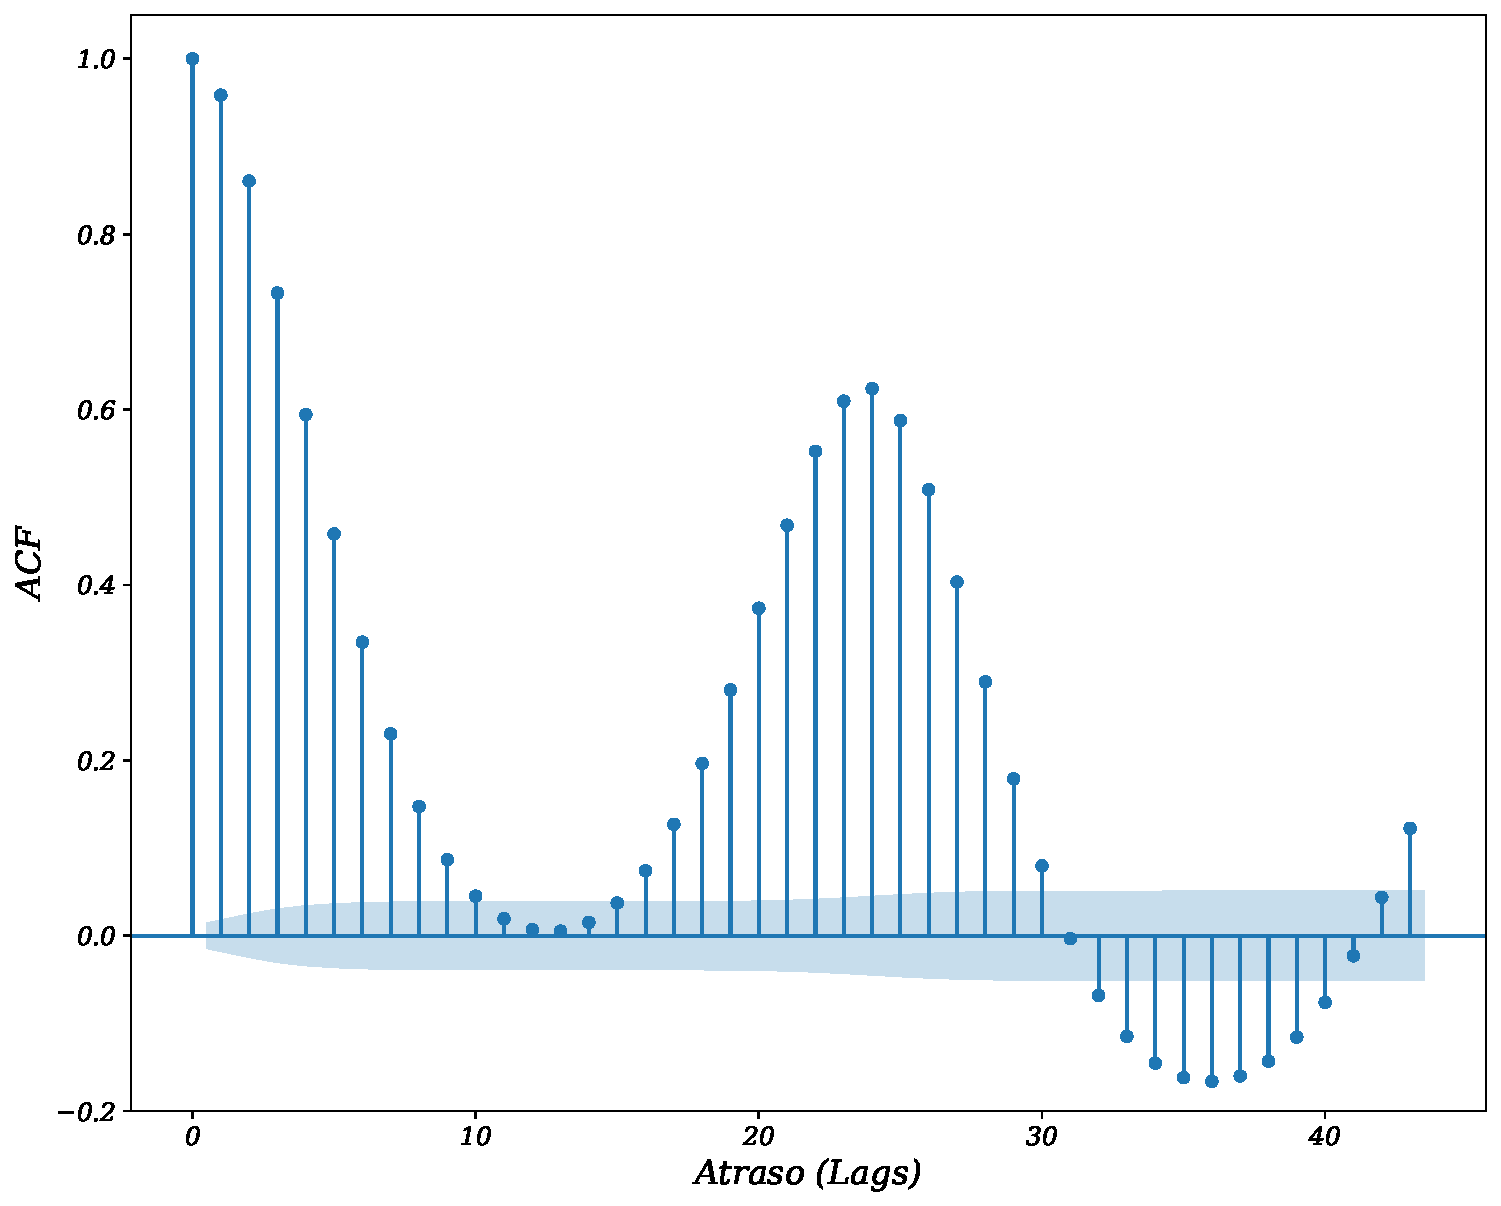
\includegraphics[width=0.7\linewidth]{Resultados/Figuras/acf} 
	
	
\end{figure}


\begin{figure}[!htb]
	\centering
	\caption{Autocorrelação parcial}\label{fig:pacf}
	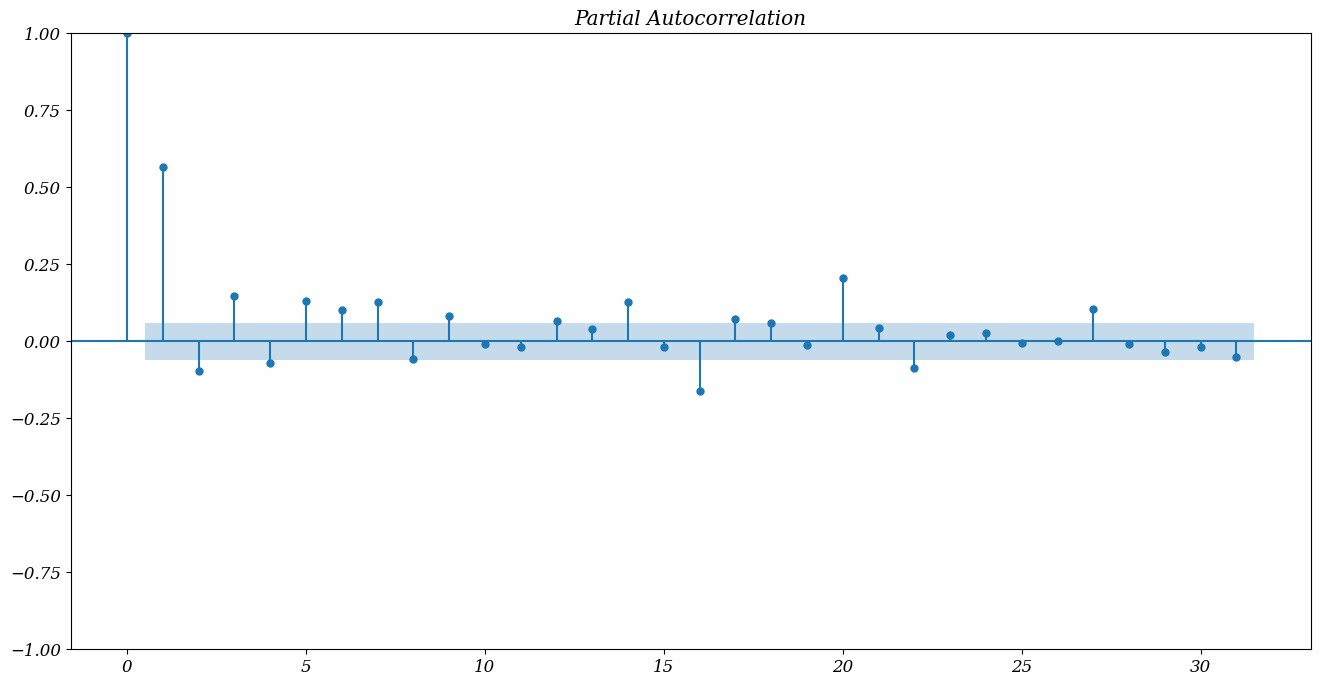
\includegraphics[width=0.7\linewidth]{Resultados/Figuras/pacf}
	
	
	
\end{figure}



Demonstrar que uma série temporal tem ou pode ter um ruído branco também é conveniente para a análise da EDA.
Na Figura \ref{fig:ruido-branco}, é possível observar uma série temporal que pode ser caracterizada como ruído branco. Uma série temporal é considerada ruído branco se suas variáveis forem independentes e distribuídas de forma idêntica, com média zero. Isso implica que todas as variáveis possuem a mesma variância ($\sigma^2$) e que cada valor não possui correlação com os demais valores da série.

\begin{figure}[!htb]
	\centering
	\caption{Ruído branco}
	\label{fig:ruido-branco}
	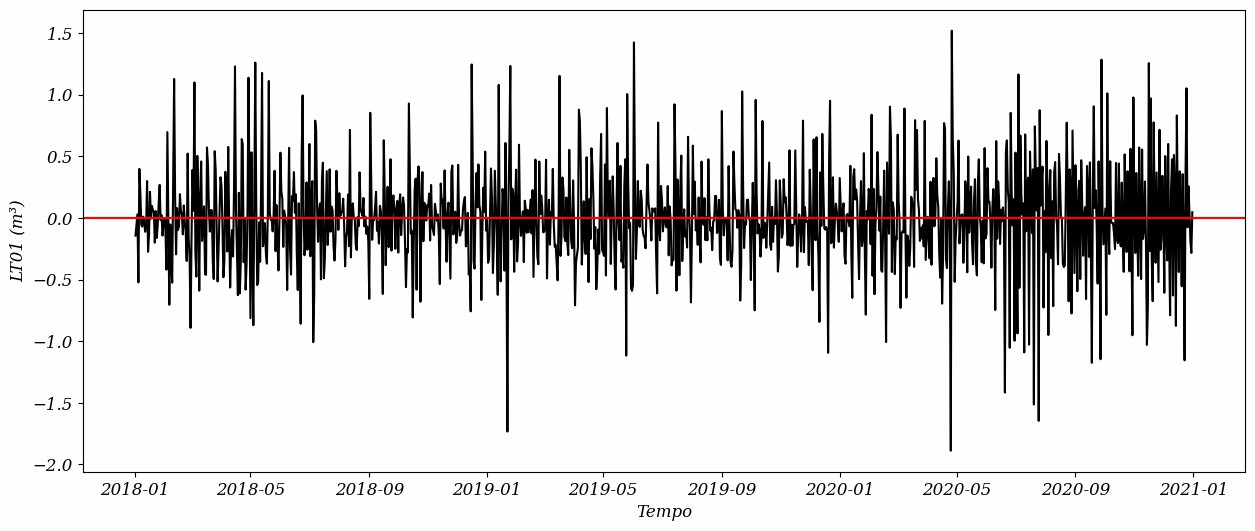
\includegraphics[width=\linewidth]{Resultados/Figuras/ruido-branco}
	
	
\end{figure}

Nesse exemplo, ao utilizar os dados da SANEPAR, a série temporal trabalhada é estacionária e também apresenta ruído branco (do inglês \textit{white noise}).



Com base na forte evidência contra a hipótese nula, podemos rejeitar a hipótese nula. A Figura \ref{fig:hist}, podemos notar um aumento na demanda durante essas horas durante o ano de 2019.
Conforme mencionado na subseção \ref{subsubsec:motivacao}, as anomalias climáticas ocorridas em 2020, especialmente a falta de chuvas e devido ao COVID-19, tiveram um impacto significativo nos resultados. Isso contribuiu para as mudanças observadas na demanda de água ao longo desse período.

\begin{figure}[!htb]
	\centering
	\caption{Violino no nível do reservatório}
	\label{fig:hist}
	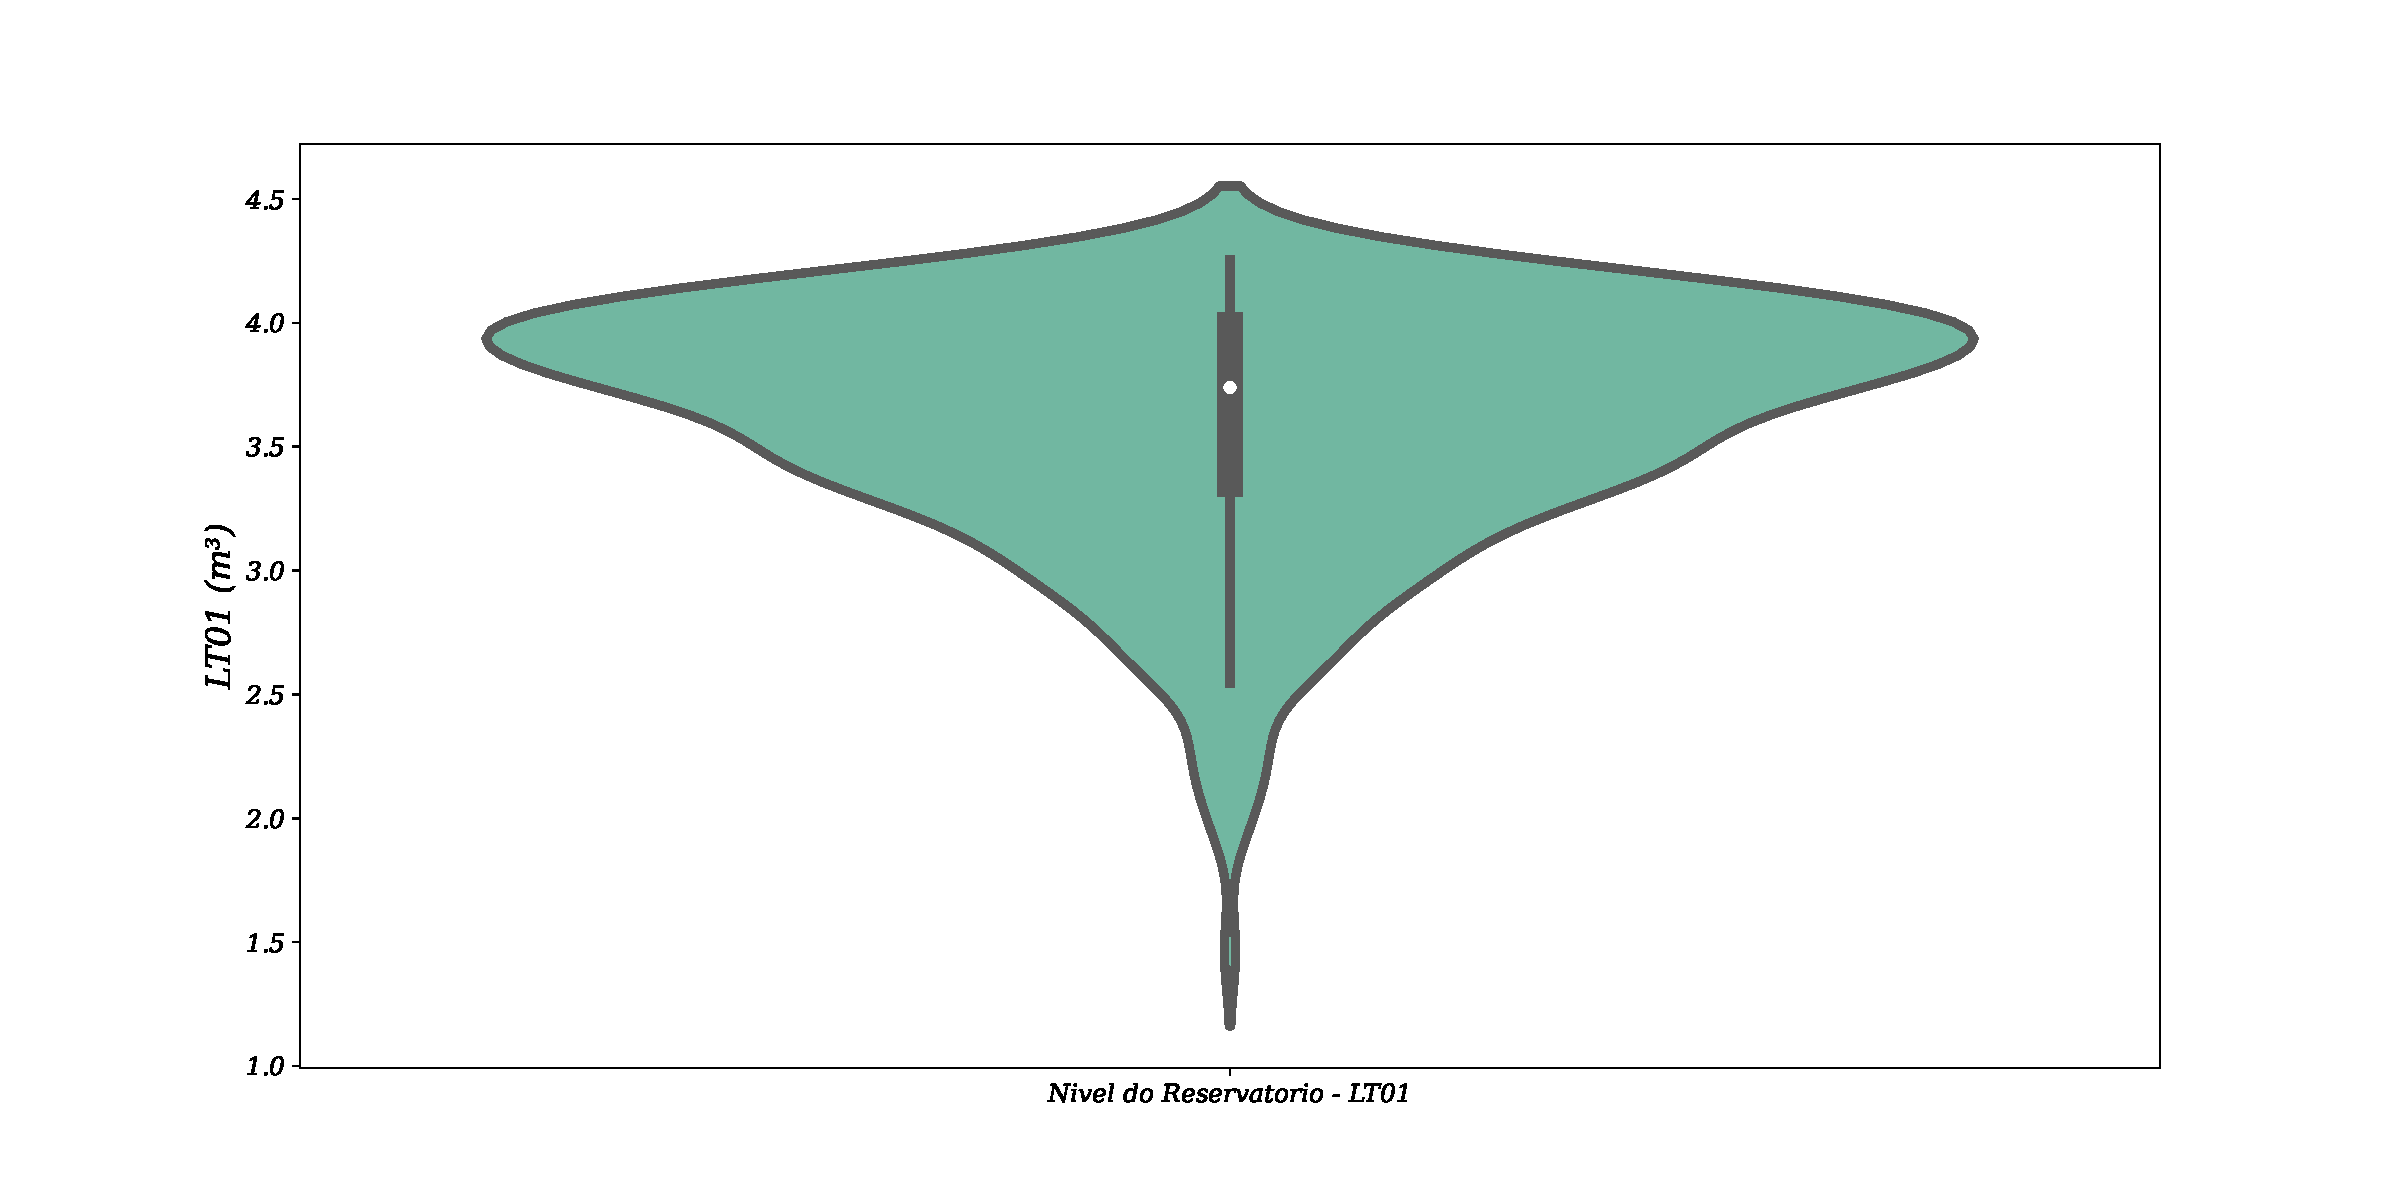
\includegraphics[width=0.7\linewidth]{Resultados/Figuras/viol}
	
	
\end{figure}





A Figura \ref{fig:ft03} mostra como a vazão pode ser afetada pelo nível do tanque. É interessante observar que a vazão de recalque tem um impacto mais significativo no nível do tanque em comparação com as outras vazões. Isso ocorre porque a vazão de recalque está associada à injeção de água diretamente no tanque por meio da bomba localizada próxima à base do tanque. Por outro lado, as demais vazões apresentam alguns valores ausentes, o que limita sua influência na análise geral.	


\begin{figure}[!htb]
	\centering
	\caption{Violino da vazão de recalque}
	\label{fig:ft03}
	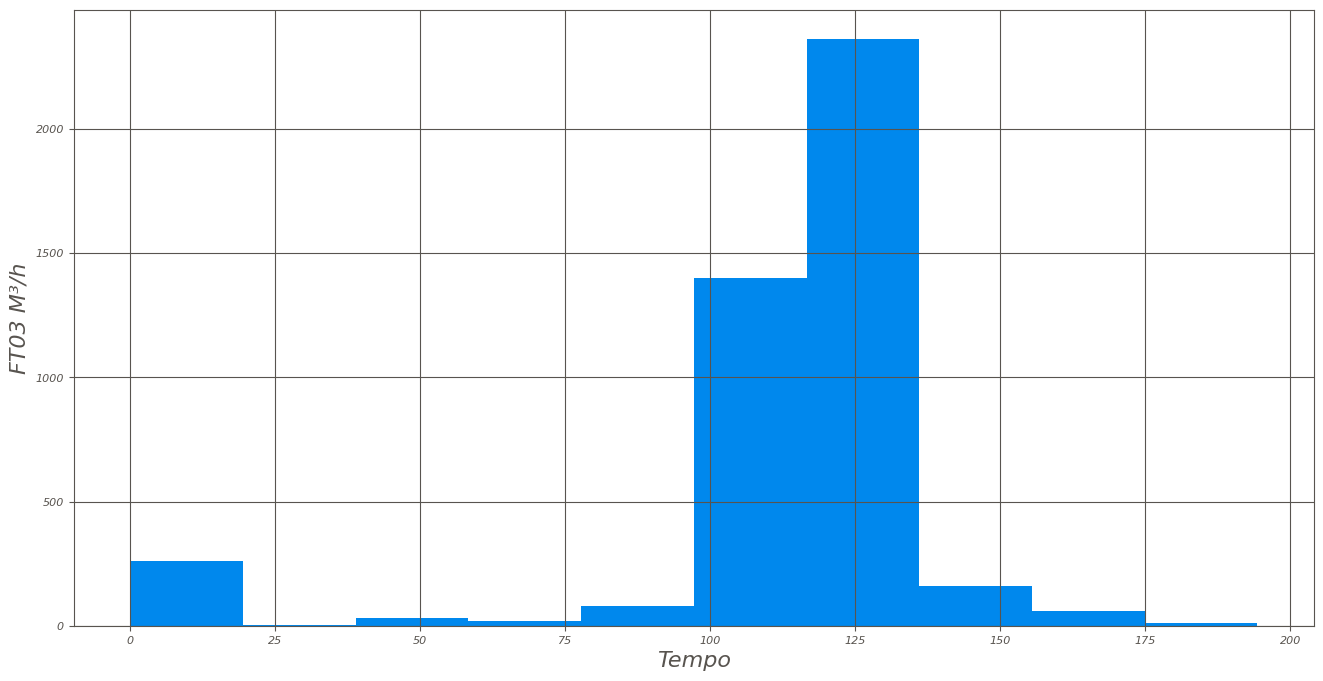
\includegraphics[width=0.7\linewidth]{Resultados/Figuras/ft03}
	
	
\end{figure}




